\label{part3}
Les résultats que nous avons eus sont présentés en deux étapes. Tout d'abord, les résultats de YOLO V5 sur notre jeu de données ont été très précis et ont répondu positivement à nos attentes. En effet, en une centaine d'epochs d'entraînement, YOLO V5 présentait sur notre jeu de données une précision avoisinant les 92\% pour la reconnaissance de globules blancs. 

\begin{figure}[!h]
    \centering
    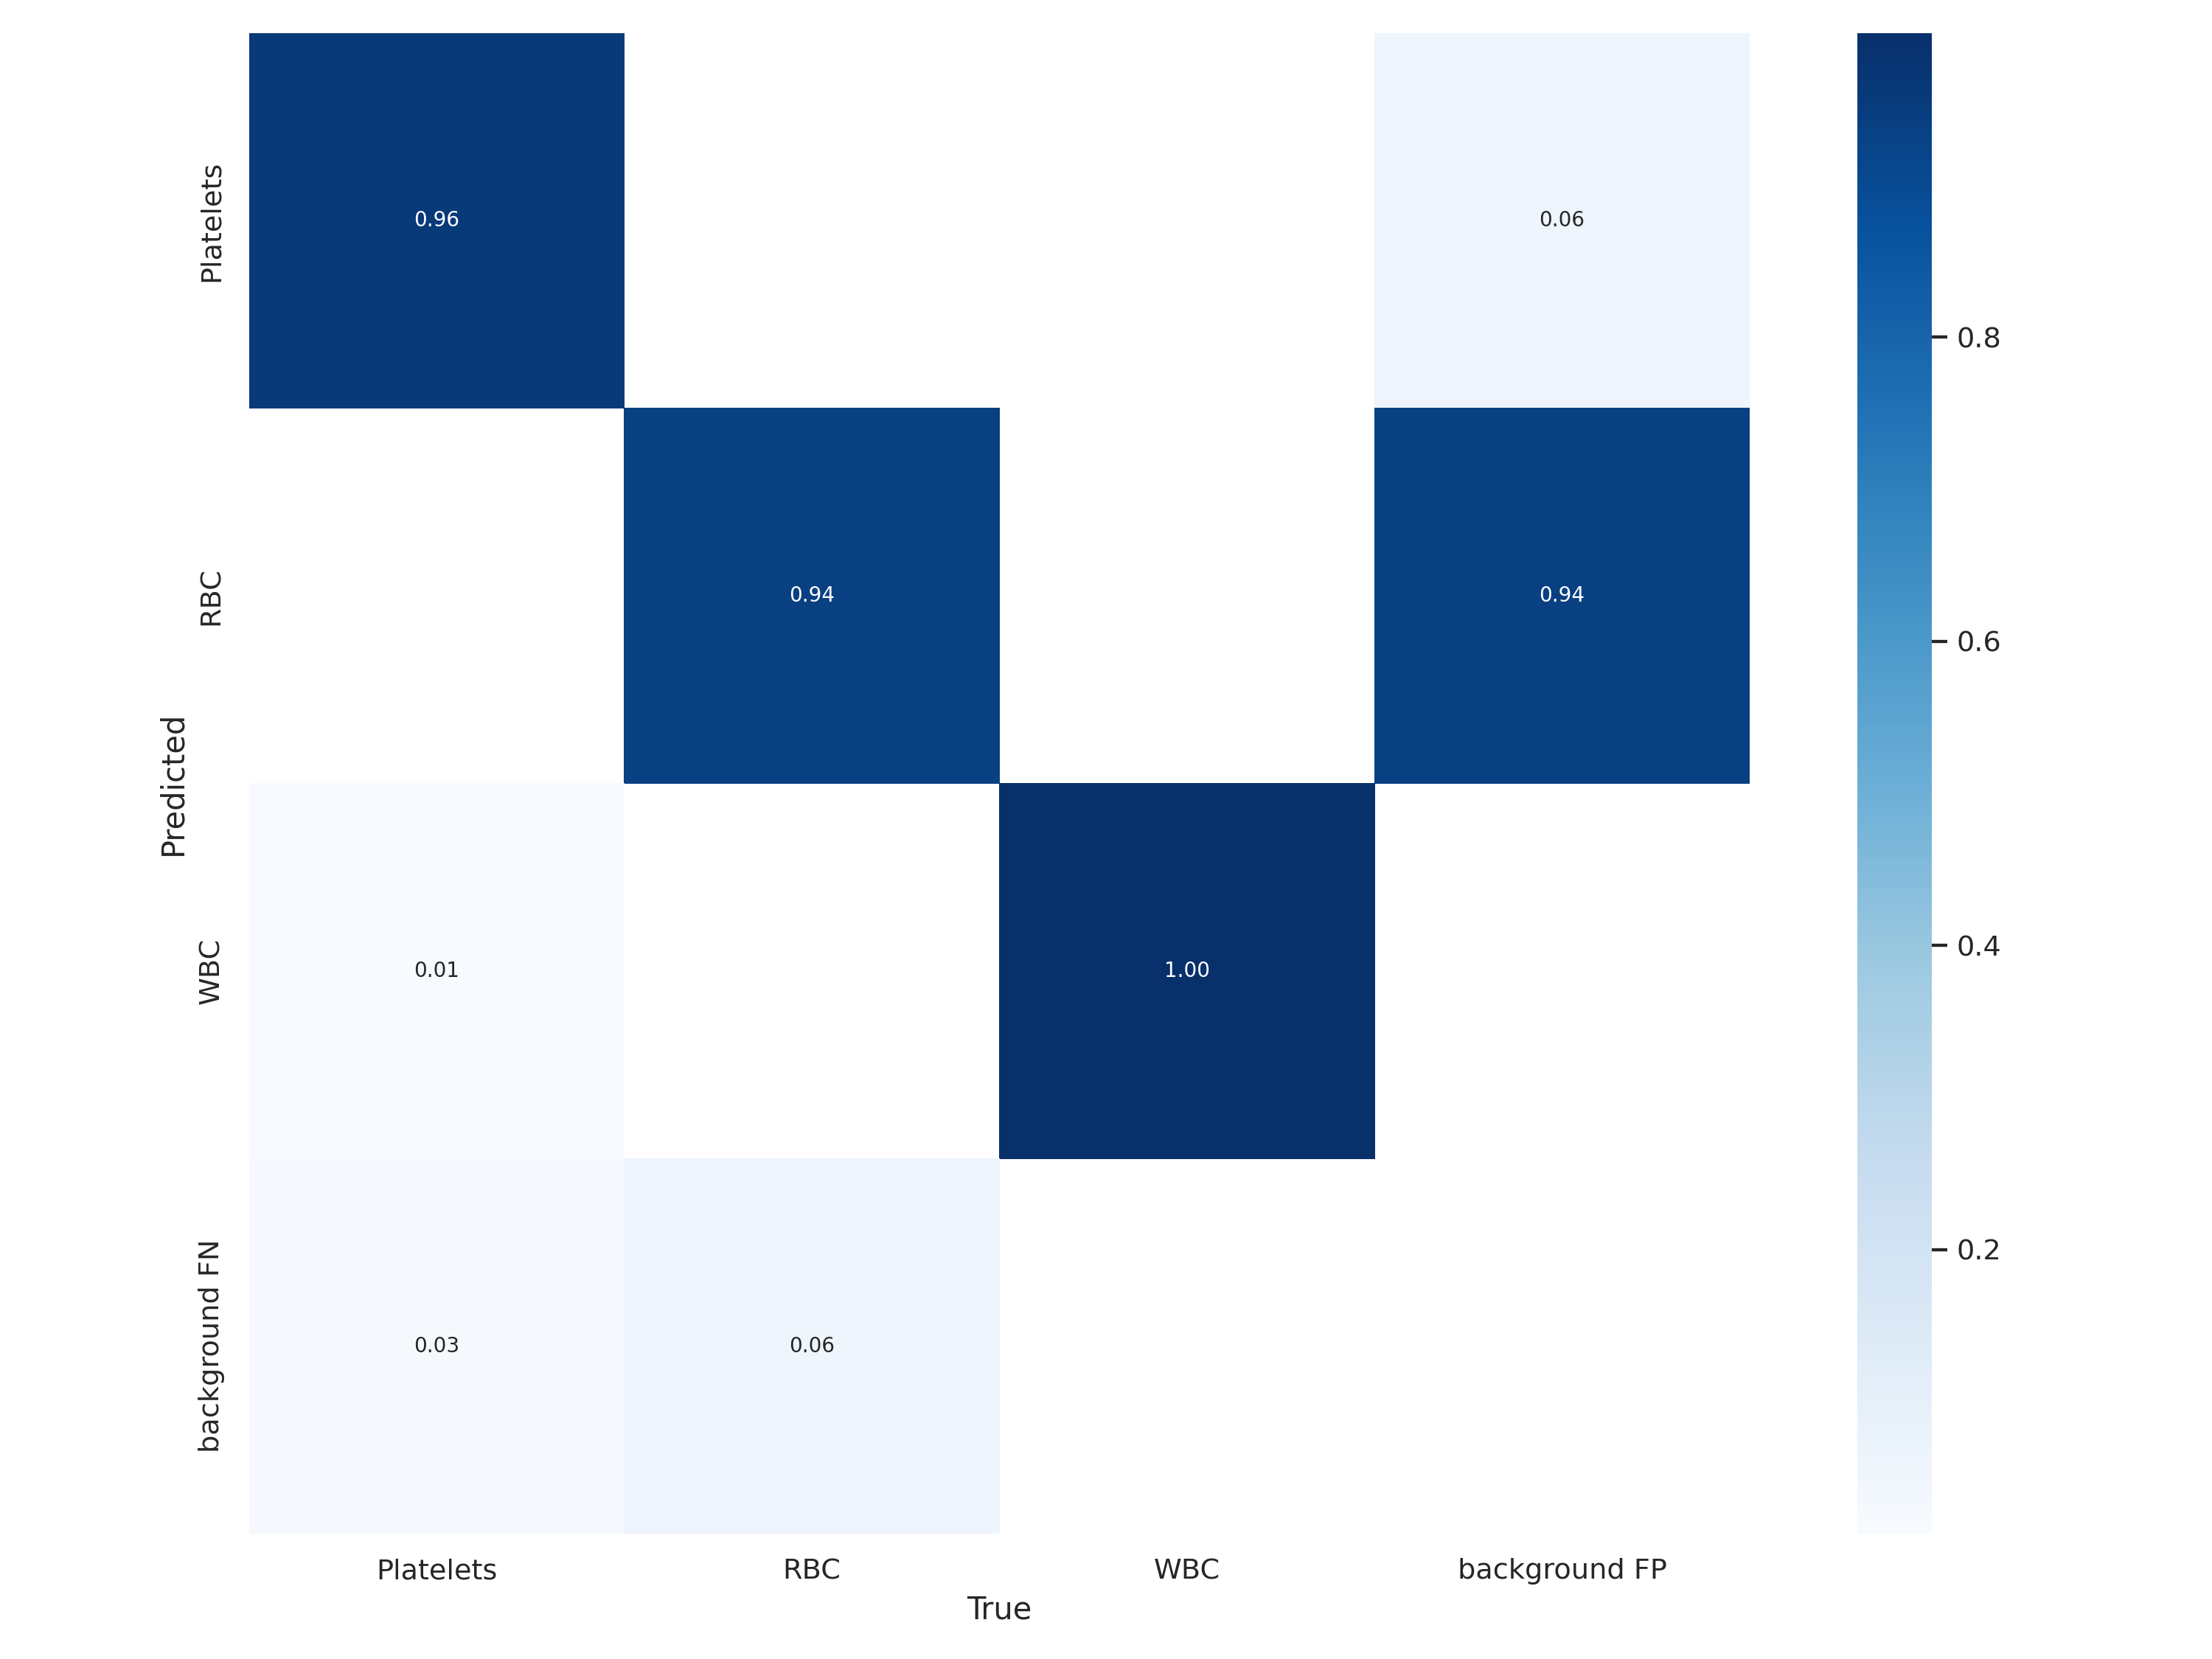
\includegraphics[scale=0.22]{images/confusion_matrix.png}
    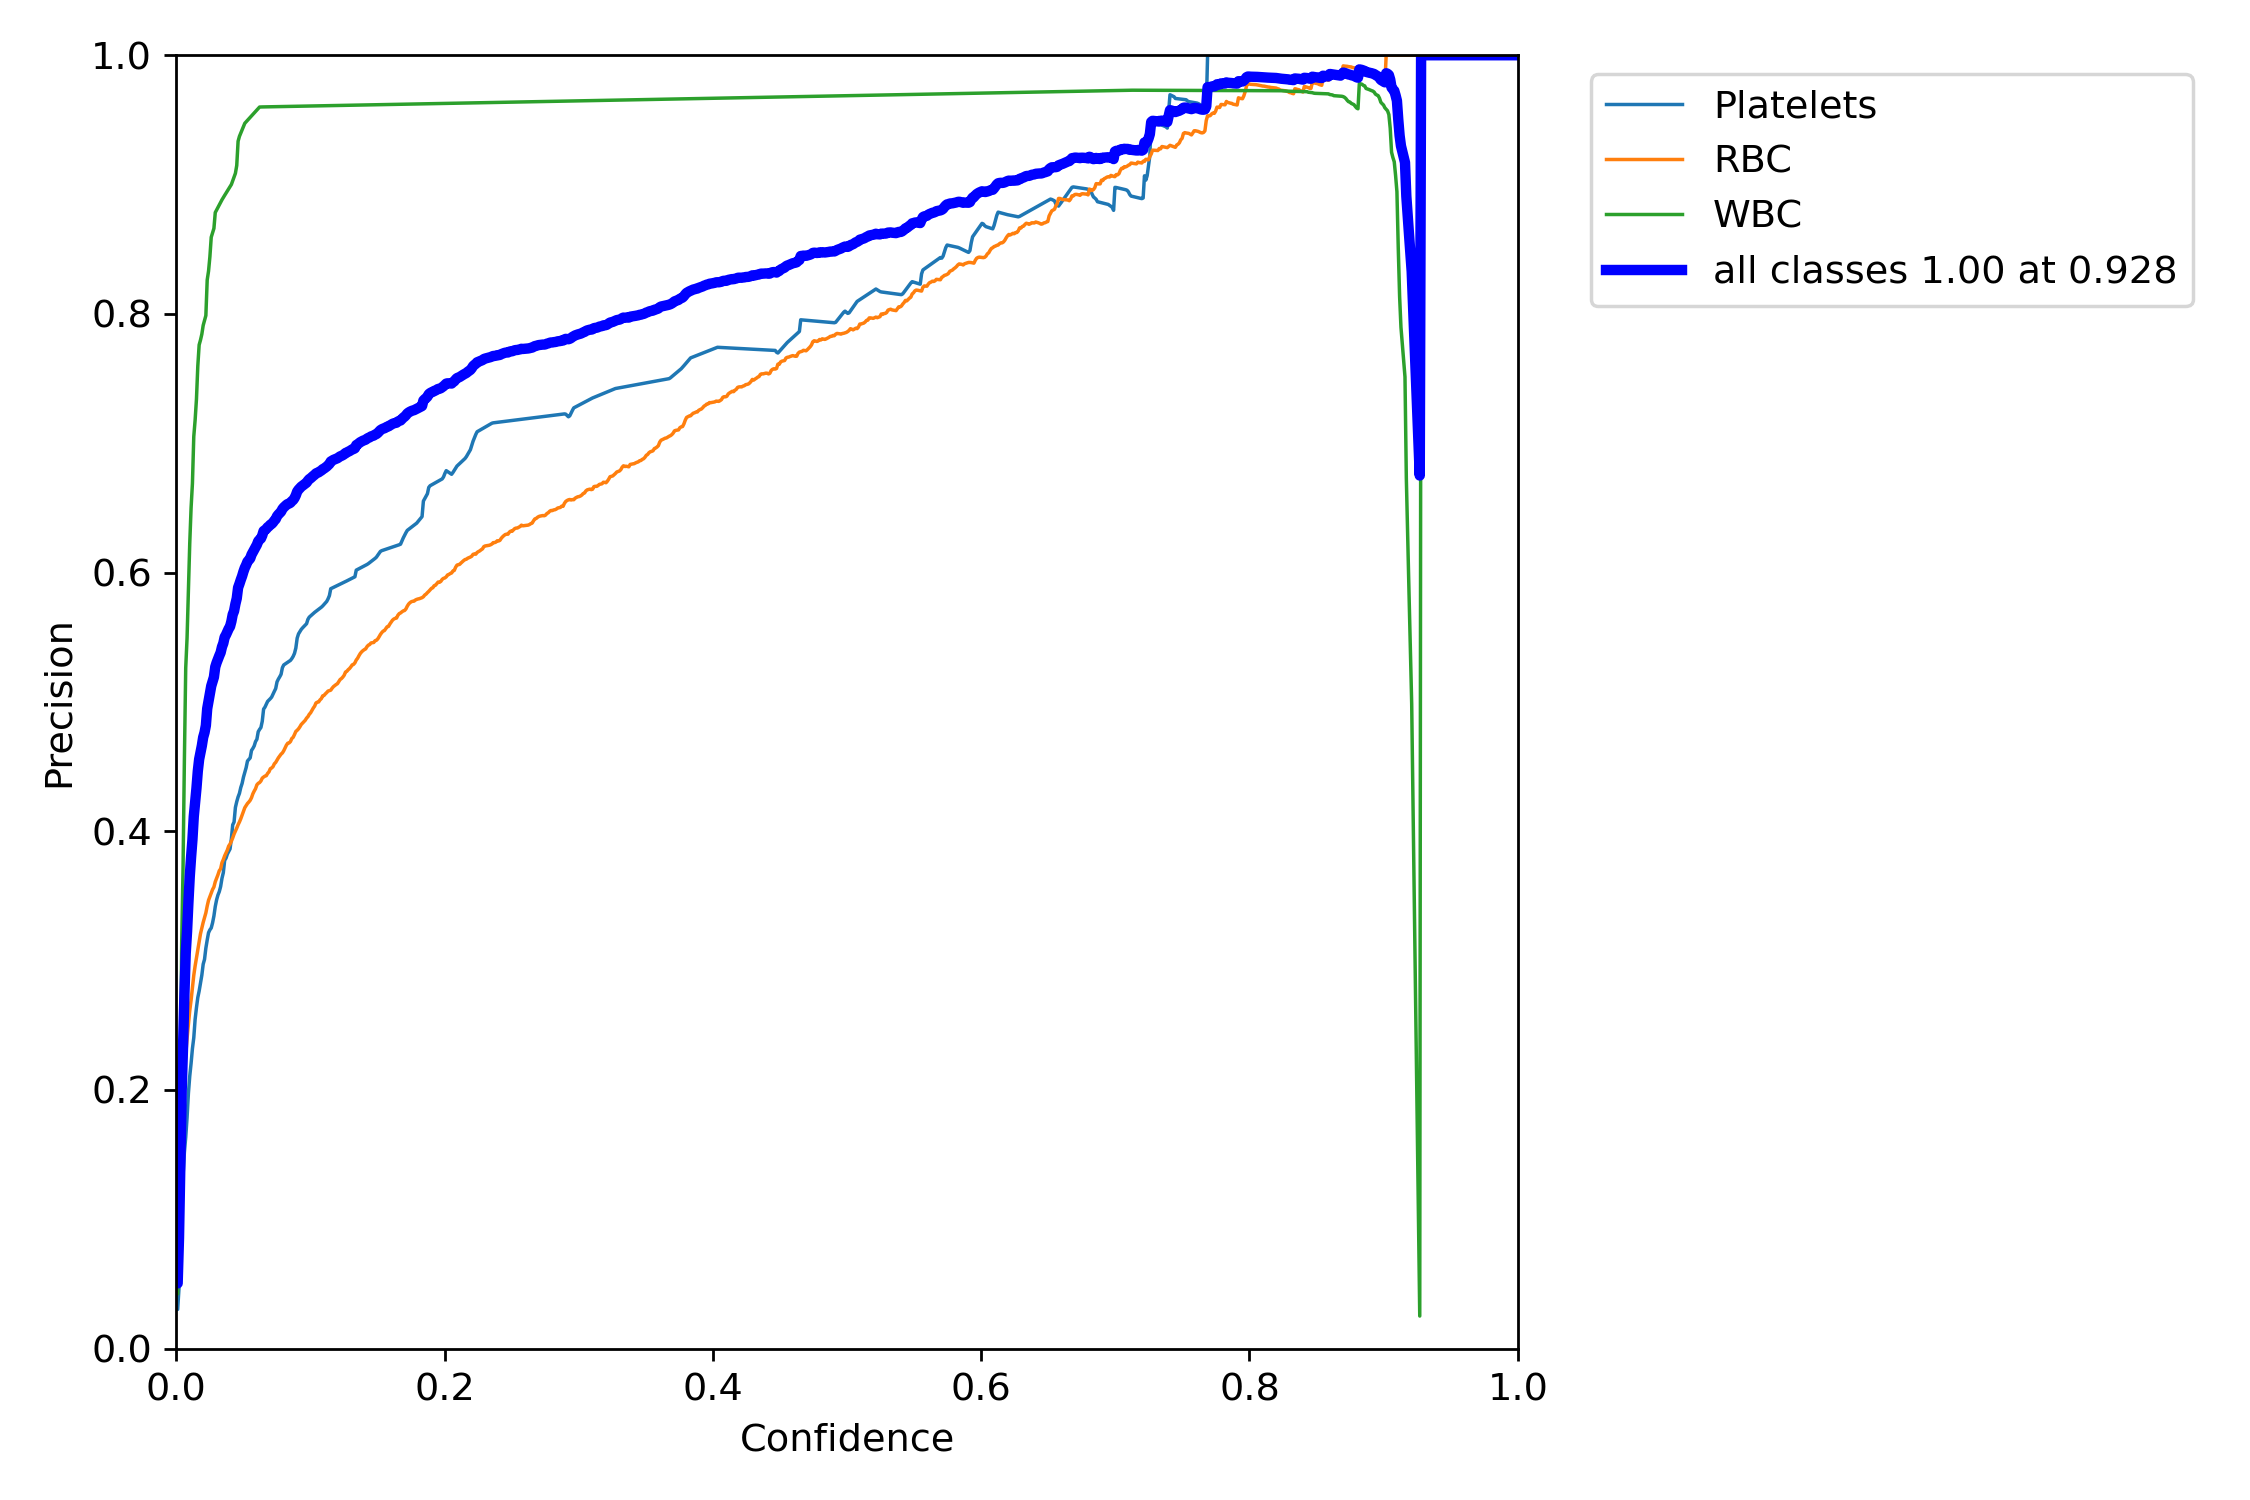
\includegraphics[scale=0.35]{images/precision_confidence.png}
    \caption{Matrice de confusion}
    \caption{Rapport précision sur confiance}
    \label{fig:matrice-precision}
\end{figure}

\paragraph{}
Nous avons considéré que les résultats obtenus étaient suffisamment satisfaisant pour ne pas nécessiter d'approfondir ou d'améliorer l'algorithme, et nous avons donc procédé à la réalisation de l'algorithme de découpage puis du CNN pour l'étape finale du projet.
Pour l'application du jeu de données au CNN final, les résultats présentés sont d'une précision de 95\% en une centaine d'epochs d'entraînement.